\documentclass{standalone}[9pt]
% main document, called main.tex
\usepackage{tikz}
\usetikzlibrary{external}
\usetikzlibrary{arrows,shapes,backgrounds,decorations.pathreplacing}
\tikzexternalize % activate!
\begin{document}
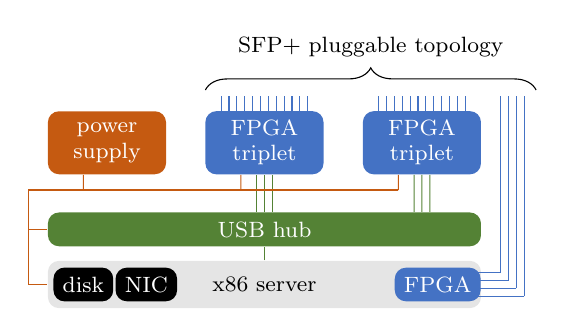
\begin{tikzpicture}
  [scale=.5,auto=left,every node/.style={rectangle,rounded
     corners,fill=myblue,text=white},align=center]
  \definecolor{myblue}{RGB}{68,114,196}
  \definecolor{myorange}{RGB}{197,90,17}
  \definecolor{myorange}{RGB}{197,90,17}
  \definecolor{mygreen}{RGB}{84,130,53}

  \node[fill=myorange,minimum width=1.5cm,minimum height=0.8cm] (power) at (0,0)
     {\footnotesize{power}\\[-1mm]\footnotesize{supply}};
  \node[minimum width=1.5cm,minimum height=0.8cm] (triplet1) at (4,0)
     {\footnotesize{FPGA}\\[-1mm]\footnotesize{triplet}};
  \node[minimum width=1.5cm,minimum height=0.8cm] (triplet2) at (8,0)
     {\footnotesize{FPGA}\\[-1mm]\footnotesize{triplet}};

  \node[fill=mygreen,minimum width=5.5cm] (hub)
     at (4,-2.2)
     {\footnotesize{USB hub}};

  \draw[arrows=-,>=stealth,color=mygreen]
    ([xshift=-2mm]hub.north) to ([xshift=-2mm]triplet1.south);
  \draw[arrows=-,>=stealth,color=mygreen]
    ([xshift=-0mm]hub.north) to ([xshift=0mm]triplet1.south);
  \draw[arrows=-,>=stealth,color=mygreen]
    ([xshift=2mm]hub.north) to ([xshift=2mm]triplet1.south);
 
  \draw[arrows=-,>=stealth,color=mygreen]
    ([xshift=38mm]hub.north) to ([xshift=-2mm]triplet2.south);
  \draw[arrows=-,>=stealth,color=mygreen]
    ([xshift=40mm]hub.north) to ([xshift=0mm]triplet2.south);
  \draw[arrows=-,>=stealth,color=mygreen]
    ([xshift=42mm]hub.north) to ([xshift=2mm]triplet2.south);
 
  \node[fill=gray!20,text=black,minimum width=5.5cm,minimum height=0.6cm] (x86)
     at (4,-3.6) {\footnotesize{x86 server}};

  \node[fill=myblue] (bridge)
     at (8.4,-3.6) {\footnotesize{FPGA}};

  \node[fill=black] (disk)
     at (-0.6,-3.6) {\footnotesize{disk}};

  \node[fill=black] (ethernet)
     at (1,-3.6) {\footnotesize{NIC}};

  \draw[arrows=-,>=stealth,color=mygreen]
    (x86.north) to (hub.south);

  %\draw[arrows=-,>=stealth,color=myorange]
  %  ([yshift=-6mm]power.east) to (x86.west);

  %\draw[arrows=-,>=stealth,color=myorange]
  %  ([yshift=8mm]power.east) to (hub.west);

  \coordinate[] (junc) at (-2,-1.2) {};

  %\draw[arrows=-,>=stealth,color=myorange]
  %  (power.north) to (junc);

  \coordinate[] (junc1) at (-0.6,-1.2) {};

  \draw[arrows=-,>=stealth,color=myorange]
    (junc) to (junc1);
  \draw[arrows=-,>=stealth,color=myorange]
    (junc1) to ([xshift=-6mm]power.south);

  \coordinate[] (junc2) at (3.4,-1.2) {};
  \draw[arrows=-,>=stealth,color=myorange]
    (junc1) to (junc2);
  \draw[arrows=-,>=stealth,color=myorange]
    (junc2) to ([xshift=-6mm]triplet1.south);


  \coordinate[] (junc3) at (7.4,-1.2) {};
  \draw[arrows=-,>=stealth,color=myorange]
    (junc2) to (junc3);
  \draw[arrows=-,>=stealth,color=myorange]
    (junc3) to ([xshift=-6mm]triplet2.south);

  \coordinate[] (junc4) at (-2,-2.2) {};
  \draw[arrows=-,>=stealth,color=myorange]
    (junc) to (junc4);
  \draw[arrows=-,>=stealth,color=myorange]
    (junc4) to (hub.west);

  \coordinate[] (junc5) at (-2,-3.6) {};
  \draw[arrows=-,>=stealth,color=myorange]
    (junc4) to (junc5);
  \draw[arrows=-,>=stealth,color=myorange]
    (junc5) to (x86.west);


  %\node[fill=none,text=black] (internet)
  %   at (1,-5) {\footnotesize{internet}};
  %\draw[arrows=<->,>=stealth,color=black]
  % (internet.north) to (ethernet.south);

  \coordinate[] (net) at (4, 1.2) {};
  \draw[arrows=-,>=stealth,color=myblue]
    ([xshift=-1mm]triplet1.north) to ([xshift=-1mm]net);
  \draw[arrows=-,>=stealth,color=myblue]
    ([xshift=-3mm]triplet1.north) to ([xshift=-3mm]net);
  \draw[arrows=-,>=stealth,color=myblue]
    ([xshift=-5mm]triplet1.north) to ([xshift=-5mm]net);
  \draw[arrows=-,>=stealth,color=myblue]
    ([xshift=-7mm]triplet1.north) to ([xshift=-7mm]net);
  \draw[arrows=-,>=stealth,color=myblue]
    ([xshift=-9mm]triplet1.north) to ([xshift=-9mm]net);
  \draw[arrows=-,>=stealth,color=myblue]
    ([xshift=-11mm]triplet1.north) to ([xshift=-11mm]net);
  \draw[arrows=-,>=stealth,color=myblue]
    ([xshift=1mm]triplet1.north) to ([xshift=1mm]net);
  \draw[arrows=-,>=stealth,color=myblue]
    ([xshift=3mm]triplet1.north) to ([xshift=3mm]net);
  \draw[arrows=-,>=stealth,color=myblue]
    ([xshift=5mm]triplet1.north) to ([xshift=5mm]net);
  \draw[arrows=-,>=stealth,color=myblue]
    ([xshift=7mm]triplet1.north) to ([xshift=7mm]net);
  \draw[arrows=-,>=stealth,color=myblue]
    ([xshift=9mm]triplet1.north) to ([xshift=9mm]net);
  \draw[arrows=-,>=stealth,color=myblue]
    ([xshift=11mm]triplet1.north) to ([xshift=11mm]net);

  \coordinate[] (netR) at (8, 1.2) {};
  \draw[arrows=-,>=stealth,color=myblue]
    ([xshift=-1mm]triplet2.north) to ([xshift=-1mm]netR);
  \draw[arrows=-,>=stealth,color=myblue]
    ([xshift=-3mm]triplet2.north) to ([xshift=-3mm]netR);
  \draw[arrows=-,>=stealth,color=myblue]
    ([xshift=-5mm]triplet2.north) to ([xshift=-5mm]netR);
  \draw[arrows=-,>=stealth,color=myblue]
    ([xshift=-7mm]triplet2.north) to ([xshift=-7mm]netR);
  \draw[arrows=-,>=stealth,color=myblue]
    ([xshift=-9mm]triplet2.north) to ([xshift=-9mm]netR);
  \draw[arrows=-,>=stealth,color=myblue]
    ([xshift=-11mm]triplet2.north) to ([xshift=-11mm]netR);
  \draw[arrows=-,>=stealth,color=myblue]
    ([xshift=1mm]triplet2.north) to ([xshift=1mm]netR);
  \draw[arrows=-,>=stealth,color=myblue]
    ([xshift=3mm]triplet2.north) to ([xshift=3mm]netR);
  \draw[arrows=-,>=stealth,color=myblue]
    ([xshift=5mm]triplet2.north) to ([xshift=5mm]netR);
  \draw[arrows=-,>=stealth,color=myblue]
    ([xshift=7mm]triplet2.north) to ([xshift=7mm]netR);
  \draw[arrows=-,>=stealth,color=myblue]
    ([xshift=9mm]triplet2.north) to ([xshift=9mm]netR);
  \draw[arrows=-,>=stealth,color=myblue]
    ([xshift=11mm]triplet2.north) to ([xshift=11mm]netR);

  \draw [decorate,rotate=270,decoration={brace,amplitude=8pt},
       xshift=-4pt,yshift=0pt]
  (-1.2,2.5) -- (-1.2,10.9) node [yshift=3mm,midway,fill=none,text=black] 
  {\footnotesize{SFP+ pluggable topology}};

  \coordinate[] (bridge0) at (10, -3.6);
  \draw[arrows=-,>=stealth,color=myblue]
    ([yshift=3mm,xshift=-2mm]bridge.east) to ([yshift=3mm]bridge0.west);
  \draw[arrows=-,>=stealth,color=myblue]
    ([yshift=1mm,xshift=-1mm]bridge.east) to
    ([xshift=2mm,yshift=1mm]bridge0.west);
  \draw[arrows=-,>=stealth,color=myblue]
    ([yshift=-1mm,xshift=-1mm]bridge.east) to
    ([xshift=4mm,yshift=-1mm]bridge0.west);
  \draw[arrows=-,>=stealth,color=myblue]
    ([yshift=-3mm,xshift=-2mm]bridge.east) to
    ([xshift=6mm,yshift=-3mm]bridge0.west);

  \coordinate[] (bridge1) at (10, 1.2);
  \draw[arrows=-,>=stealth,color=myblue]
    ([yshift=3mm]bridge0.north) to (bridge1.south);
  \draw[arrows=-,>=stealth,color=myblue]
    ([yshift=1mm,xshift=2mm]bridge0.north) to ([xshift=2mm]bridge1.south);
  \draw[arrows=-,>=stealth,color=myblue]
    ([yshift=-1mm,xshift=4mm]bridge0.north) to ([xshift=4mm]bridge1.south);
  \draw[arrows=-,>=stealth,color=myblue]
    ([yshift=-3mm,xshift=6mm]bridge0.north) to ([xshift=6mm]bridge1.south);

\end{tikzpicture}
\end{document}
